\label{sec:experiments}
The experiments address three questions: how COMPASS source models respond to
preserving rewrites, how independently adapted text encoders affect retrieval,
and whether internal diagnostics support the proposed stability mechanism.
We report generation quality and retrieval for explicitly distinguished
configurations, then examine component choices, text-domain transfer, and
hidden-state behavior.

\subsection{Experimental Setup}
\label{sec:independent_adaptation}
\label{sec:detail_protocol_details}

\paragraph{Datasets and prompt pairs.}
We use HumanML3D~\cite{guo2022generating}, Motion-X~\cite{lin2023motionx}, and
KIT-ML~\cite{plappert2016kit}, with native 263-, 322-, and 251-dimensional
motion representations. Preserving rewrites are grouped into lexical changes
(P1), syntactic changes (P2), and narrative-style changes (P3). The mixed
HumanML3D and Motion-X tests contain 4,380 and 7,679 caption-locked motions:
each motion has a fixed original caption, rewrite, and crop. Before testing,
seed 123 assigns one rewrite per motion, giving P1/P2/P3 counts of
1,460/1,460/1,460 and 2,560/2,560/2,559. Each mixture is evaluated as a
single dataset, rather than by averaging level-specific metrics.
Native KIT retains 734 full-motion pairs from 830 entries under its native
length rules. The separate 734-pair transfer set uses the archived P2/P3
pairing; it is not interchangeable with the native mixture. Pair order,
normalization, and source checkpoints are fixed before generation.

\paragraph{Source and adapted configurations.}
A \emph{source configuration} uses each model's text encoder before the
additional text-only adaptation stage. An \emph{adapted configuration} updates
that model's native text encoder: CLIP for the T2M-GPT family and T5 for the
MotionGPT family. Encoders are independent across models. The FID variants in
the mixed-result tables use source configurations; every other column,
including retrieval, Matching, diversity, and transfer pair/token measures,
uses adapted configurations. Both share prompts, generation settings, and the
frozen motion evaluator, but generate separate actions. The column-wise
reporting was revised after inspection of the adapted results. Both complete
result sets are retained. The T2M-GPT+COMPASS source checkpoint was
subsequently reselected from a sweep of thirteen training endpoints scored on
this mixture, so that row is a test-selected endpoint and its margins are
optimistic; all other rows retain their pre-declared endpoints.

\paragraph{Text-only adaptation.}
Each native text encoder receives 3,000 updates with equal-weight
original/rewrite action-token prediction on training-only preserving pairs.
The generation backbone, VQ-VAE, auxiliary heads, and CLIP visual branch remain
frozen; for T5, the shared embeddings, decoder, and output layer also remain
frozen. This stage does not reapply COMPASS losses. HumanML3D, KIT, and component
variants use learning rate $10^{-6}$, 100 warmup steps, and a fixed endpoint.
Motion-X retains the previously validation-selected configurations, including
T5 learning rates $3\times10^{-5}$ for MotionGPT and $10^{-6}$ for
MotionGPT+COMPASS. Only matching training annotations and valid native motion
tokens are admitted; held-out motions and mirrored sources are excluded.
The Motion-X MotionGPT+COMPASS source is the preserve-only variant described in
the method. Component sources retain their differing original training budgets.

\paragraph{Generation.}
Every test uses generation seed 123 and CFG $s=1.3$, applied to conditional
and unconditional logits as $\ell_u+s(\ell_c-\ell_u)$. Original and rewritten
conditions reset the same deterministic per-batch random seed. T2M-GPT uses
zero CLIP features for its unconditional branch. For MotionGPT, an
inference-time branch retains \texttt{Generate motion:} but removes the
description and uses the same decoder prefix. At CFG=1, the wrapper reproduces
the original MotionGPT generation path. This extension does not imply that
these T5 checkpoints were trained with unconditional-caption dropout, and the
two architectures have different unconditional inputs. Native motion
tokenizers, length rules, and normalization are preserved, including KIT's
251-dimensional representation at 12.5 frames per second.

\paragraph{Shared evaluators.}
All models within a dataset use the same frozen text--motion matching
evaluator. Its text encoder is adapted to training clean/preserving pairs;
its movement and motion encoders retain standard weights. Word lookup first
tries the original form and falls back to lowercase only on failure.
HumanML3D and KIT retain alphabetic-token filtering; Motion-X retains its
non-alphabetic-inclusive processing. Evaluator adaptation and lookup correction
are distinct from adapting the generator's CLIP or T5 encoder.

For KIT evaluator selection, 288 eligible official validation motions provide
864 P1/P2/P3 rewrites generated and filtered with \texttt{gemini-3.1-flash-lite}.
These texts are used only for validation. Evaluator text training uses 20
rounds of 200 updates at learning rate $10^{-4}$; a batch contains eight
unique motions, each with clean/P1/P2/P3 text, and rolled negatives from
different motions. The predeclared acceptance criteria allow at most a
one-percentage-point clean R@1 drop, require a macro rewrite R@1 gain of at
least 0.5 points, and require P3 nonregression. Round 20 is selected: clean
R@1 increases from 42.53\% to 43.77\%, and macro rewrite R@1 from 26.00\%
to 39.18\%. These are real-motion validation scores, not generator gains.
Motion-side parameter hashes and save/reload consistency are verified.

% Float placement policy: each wide table is declared roughly one subsection
% ahead of the text that discusses it. IEEE two-column table* floats can only
% reach the top of a later page, so declaring them at the point of discussion
% pushed them one to two pages downstream.
\begin{table*}[t]
\centering
\caption{HumanML3D on 4,380 fixed prompt pairs, CFG=1.3. FID variants use source encoders; other columns use adapted encoders and separate generations. Retrieval (\%) averages 20 candidate partitions of one generation seed. Bold marks the within-family best; diversity is closest to the real reference (9.137).}
\label{tab:humanml_methods}
\resulttablesetup
\begin{tabular*}{\textwidth}{@{\extracolsep{\fill}}l*{8}{c}@{}}
\toprule
Method & \multicolumn{3}{c}{Source encoder} & \multicolumn{5}{c}{Adapted encoder} \\
\cmidrule(lr){2-4}\cmidrule(lr){5-9}
 & FID $\downarrow$ & FID$_P$ $\downarrow$ & FID$_D$ $\downarrow$ & Matching$_P$ $\downarrow$ & R@1$_P$ $\uparrow$ & R@2$_P$ $\uparrow$ & R@3$_P$ $\uparrow$ & Div.$_O$ \\
\midrule
T2M-GPT & \textbf{0.080} & 0.233 & 0.190 & 4.169 & 36.36 & 52.15 & 61.76 & 8.421 \\
T2M-GPT+COMPASS & 0.147 & \textbf{0.170} & \textbf{0.132} & \textbf{3.462} & \textbf{45.11} & \textbf{63.23} & \textbf{72.89} & \textbf{9.340} \\
\midrule
MotionGPT & 0.741 & 0.670 & \textbf{0.111} & 4.449 & 34.29 & 50.41 & 60.07 & \textbf{9.410} \\
MotionGPT+COMPASS & \textbf{0.516} & \textbf{0.371} & 0.167 & \textbf{4.263} & \textbf{36.09} & \textbf{52.76} & \textbf{62.29} & 9.527 \\
\bottomrule
\end{tabular*}

\end{table*}

\paragraph{Metrics and reporting.}
Fr\'echet inception distance (FID) is computed in the evaluator's motion
embedding space. FID compares original-caption generations with the real
motions, FID$_P$ compares rewrite generations with those real motions, and
FID$_D$ compares the two generated distributions. Each uses the entire fixed
mixture. Matching$_P$ is the mean Euclidean distance from each rewritten text
to the motion generated from that text. R@1/2/3$_P$ reports whether that motion
is among the top one, two, or three retrieved candidates. Queries and their
corresponding generated motions are jointly shuffled into 20 shared random
partitions, with at most 32 candidates per group and the final partial group
retained. Reported R-Precision percentages are averages across partitions of
one generation, not estimates over 20 generation seeds.

Diversity$_O$ uses original-caption generations from the adapted configuration
and a fixed seed for 300 sampled index pairs. Lower FID and Matching are
preferred; diversity is assessed by proximity to the real-motion reference.
Bold entries mark the best point estimates under each caption's comparison
rule, not statistically significant differences. FID values are compared only
within a dataset's embedding space. No generation-seed variance or paired
significance claim is reported.

\subsection{HumanML3D: Quality and Alignment}
\begin{table*}[t]
\centering
\caption{Motion-X on 7,679 fixed prompt pairs with a shared evaluator, CFG=1.3. FID variants use source encoders; other columns use adapted encoders. Bold marks the within-family best as in Table~\ref{tab:humanml_methods}; real diversity is 14.322.}
\label{tab:motionx_methods}
\resulttablesetup
\begin{tabular*}{\textwidth}{@{\extracolsep{\fill}}l*{8}{c}@{}}
\toprule
Method & \multicolumn{3}{c}{Source encoder} & \multicolumn{5}{c}{Adapted encoder} \\
\cmidrule(lr){2-4}\cmidrule(lr){5-9}
 & FID $\downarrow$ & FID$_P$ $\downarrow$ & FID$_D$ $\downarrow$ & Matching$_P$ $\downarrow$ & R@1$_P$ $\uparrow$ & R@2$_P$ $\uparrow$ & R@3$_P$ $\uparrow$ & Div.$_O$ \\
\midrule
T2M-GPT & 0.203 & 1.279 & 0.813 & 5.182 & 40.40 & 57.88 & 67.79 & 14.232 \\
T2M-GPT+COMPASS & \textbf{0.166} & \textbf{0.804} & \textbf{0.586} & \textbf{5.110} & \textbf{41.00} & \textbf{58.79} & \textbf{68.75} & \textbf{14.398} \\
\midrule
MotionGPT & \textbf{2.618} & 3.750 & 0.596 & 7.553 & 21.60 & 34.80 & 44.23 & \textbf{13.134} \\
MotionGPT+COMPASS & 2.775 & \textbf{3.338} & \textbf{0.109} & \textbf{7.324} & \textbf{22.68} & \textbf{36.06} & \textbf{45.73} & 13.053 \\
\bottomrule
\end{tabular*}

\end{table*}
Table~\ref{tab:humanml_methods} shows improved rewrite quality with different
costs across backbones. With source encoders, T2M-GPT+COMPASS lowers FID$_P$
from 0.233 to 0.170 and FID$_D$ from 0.190 to 0.132, while original-caption
FID increases from 0.080 to 0.147. MotionGPT+COMPASS lowers FID from 0.741
to 0.516 and FID$_P$ from 0.670 to 0.371, but increases FID$_D$ from 0.111
to 0.167. Thus closer rewrite generations to real motion do not require a
smaller gap between original- and rewrite-generated distributions.
In the adapted configurations, R@3$_P$ increases from 61.76\% to 72.89\%
for the T2M-GPT family and from 60.07\% to 62.29\% for the MotionGPT family.

\subsection{Motion-X: Dependence on Text Adaptation}
\begin{table*}[t]
\centering
\caption{HumanML3D retrieval after independent text adaptation, CFG=1.3. Each level has 4,380 prompt--motion pairs, one generation seed, and 20 shared random candidate partitions of at most 32, with the tail retained. The rewritten text is used for both generation and retrieval. Bold marks the within-family best point estimate. Values are percentages.}
\label{tab:humanml_independent_cfg}
\resulttablesetup
% Source: ablation/humanml_independent_cfg13_20260907/humanml_summary.csv
% SHA256: 8047349e39dec33d8feff6ee551e219f219cf86722e3dbc1684028f4250bda58
% Percent; one generation seed (123), averaged over 20 random candidate partitions.
\begin{tabular*}{\textwidth}{@{\extracolsep{\fill}}ll*{9}{c}@{}}
\toprule
Method & Encoder & \multicolumn{3}{c}{P1} & \multicolumn{3}{c}{P2} & \multicolumn{3}{c}{P3} \\
\cmidrule(lr){3-5}\cmidrule(lr){6-8}\cmidrule(lr){9-11}
& & R@1 & R@2 & R@3 & R@1 & R@2 & R@3 & R@1 & R@2 & R@3 \\
\midrule
T2M-GPT & CLIP & 35.54 & 50.95 & 60.47 & 42.78 & 59.64 & 69.01 & 29.29 & 43.83 & 53.49 \\
T2M-GPT + COMPASS & CLIP & \textbf{45.14} & \textbf{63.18} & \textbf{72.93} & \textbf{50.47} & \textbf{69.87} & \textbf{79.36} & \textbf{39.04} & \textbf{56.43} & \textbf{66.36} \\
\midrule
MotionGPT & T5 & 36.95 & 53.56 & 63.30 & 37.48 & 53.84 & 63.43 & 29.60 & 44.07 & 53.43 \\
MotionGPT + COMPASS & T5 & \textbf{37.48} & \textbf{54.06} & \textbf{63.98} & \textbf{39.69} & \textbf{56.92} & \textbf{66.63} & \textbf{30.75} & \textbf{45.97} & \textbf{55.48} \\
\bottomrule
\end{tabular*}

\end{table*}
\begin{table*}[t]
\centering
\caption{Motion-X retrieval on 7,679 pairs per level, using the protocol in Table~\ref{tab:humanml_independent_cfg} and the frozen Motion-X paraphrase-aware evaluator with lowercase fallback. Bold marks the within-family best. Values are point estimates in percent, not generation-seed means and deviations.}
\label{tab:motionx_independent_cfg}
\resulttablesetup
% Source: ablation/motionx_independent_cfg13_20260907/motionx_summary.csv
% SHA256: 0b4327846b6836176df4489ac8cf78eefcab4e453d477bf6022139a2d931d0a7
% Percent; one generation seed (123), averaged over 20 random candidate partitions.
\begin{tabular*}{\textwidth}{@{\extracolsep{\fill}}ll*{9}{c}@{}}
\toprule
Method & Encoder & \multicolumn{3}{c}{P1} & \multicolumn{3}{c}{P2} & \multicolumn{3}{c}{P3} \\
\cmidrule(lr){3-5}\cmidrule(lr){6-8}\cmidrule(lr){9-11}
& & R@1 & R@2 & R@3 & R@1 & R@2 & R@3 & R@1 & R@2 & R@3 \\
\midrule
T2M-GPT & CLIP & 42.55 & 60.69 & 70.73 & 48.04 & 67.18 & 76.85 & 30.85 & 46.75 & 56.99 \\
T2M-GPT + COMPASS & CLIP & \textbf{42.60} & \textbf{60.74} & \textbf{70.78} & \textbf{48.61} & \textbf{67.92} & \textbf{77.69} & \textbf{31.92} & \textbf{48.34} & \textbf{58.66} \\
\midrule
MotionGPT & T5 & 23.11 & 36.57 & 46.26 & 24.76 & 39.23 & 49.27 & 17.05 & 28.46 & 37.13 \\
MotionGPT + COMPASS & T5 & \textbf{23.98} & \textbf{37.95} & \textbf{48.08} & \textbf{25.80} & \textbf{40.77} & \textbf{51.04} & \textbf{17.94} & \textbf{29.71} & \textbf{38.62} \\
\bottomrule
\end{tabular*}

\end{table*}
With source encoders, T2M-GPT+COMPASS improves all three FID measures in
Table~\ref{tab:motionx_methods}: FID/FID$_P$/FID$_D$ are 0.166/0.804/0.586,
compared with 0.203/1.279/0.813 for its parent. MotionGPT+COMPASS lowers
FID$_P$ from 3.750 to 3.338 and FID$_D$ from 0.596 to 0.109, while increasing
original-caption FID from 2.618 to 2.775. The adapted configurations improve
R@3$_P$ from 67.79\% to 68.75\% and from 44.23\% to 45.73\% for the
two families, respectively.

A controlled pre/post-CLIP comparison explains why configuration matters.
Holding prompts, real embeddings, evaluator, CFG, and seed fixed, the
T2M-GPT-family FID ranking reverses after independent text adaptation.
Both generation backbones remain unchanged during that stage. Recomputed
summaries match the saved embeddings, and an independent float64 FID
calculation differs by less than $10^{-6}$. The checked numerical and
reference-embedding explanations therefore do not account for the reversal.
The source FID advantage cannot be combined with adapted retrieval gains as
evidence of one jointly superior system; the complete adapted FID results
remain in the experiment archive.

\subsection{Retrieval by Rewrite Level}
\begin{table*}[t]
\centering
\caption{Native KIT-ML on 734 prompt pairs, CFG=1.3, using the shared KIT evaluator selected on official validation data. FID variants use source encoders; other columns use adapted encoders and separate generations. Bold marks the column best; diversity is closest to 11.148. Retrieval is in percent.}
\label{tab:cross_dataset}
\resulttablesetup
\begin{tabular*}{\textwidth}{@{\extracolsep{\fill}}lrrrrrrrr@{}}
\toprule
Method & FID $\downarrow$ & FID$_P$ $\downarrow$ & FID$_D$ $\downarrow$ & Matching$_P$ $\downarrow$ & R@1$_P$ $\uparrow$ & R@2$_P$ $\uparrow$ & R@3$_P$ $\uparrow$ & Div.$_O$ \\
\midrule
T2M-GPT & 0.454 & 1.330 & 1.352 & 3.543 & 34.64 & 54.05 & 65.44 & \textbf{11.308} \\
MotionGPT & 1.265 & 1.446 & \textbf{0.260} & 6.343 & 22.92 & 35.93 & 44.55 & 11.395 \\
T2M-GPT+COMPASS & \textbf{0.396} & \textbf{1.194} & 1.270 & \textbf{3.323} & \textbf{36.31} & \textbf{56.48} & \textbf{68.54} & 11.358 \\
\bottomrule
\end{tabular*}

\end{table*}
The per-level tests evaluate each rewrite type on all 4,380 HumanML3D or
7,679 Motion-X motions (Tables~\ref{tab:humanml_independent_cfg}
and~\ref{tab:motionx_independent_cfg}). They use the same adapted checkpoints,
CFG, and evaluator as the mixed-table retrieval columns. Each level has its
own prompt and candidate population, so a mixed-test score is not the macro
average of the level-specific scores.

COMPASS variants have higher retrieval point estimates than their respective
parents at every rank and rewrite level. On HumanML3D, mean P1/P2/P3 R@3
increases from 60.99\% to 72.88\% for the T2M-GPT family and from 60.06\%
to 62.03\% for the MotionGPT family. The corresponding Motion-X changes are
68.19\% to 69.04\% and 44.22\% to 45.91\%. The gains span all three
rewrite types, with larger margins for the HumanML3D T2M-GPT family. They
characterize these adapted checkpoints and do not isolate individual losses
or variability across training and generation seeds.

\subsection{Native KIT-ML Evaluation}
\begin{table*}[t]
\centering
\caption{Contextual HumanML3D component comparison on 4,380 prompt pairs. FID variants use source encoders; other columns use adapted encoders. Parent/main rows reuse Table~\ref{tab:humanml_methods}. Source budgets and endpoints differ, precluding a matched causal ablation. Bold marks the column best; diversity is closest to 9.137.}
\label{tab:main_results}
\resulttablesetup
\begin{tabular*}{\textwidth}{@{\extracolsep{\fill}}lrrrrrrrr@{}}
\toprule
Method & FID $\downarrow$ & FID$_P$ $\downarrow$ & FID$_D$ $\downarrow$ & Matching$_P$ $\downarrow$ & R@1$_P$ $\uparrow$ & R@2$_P$ $\uparrow$ & R@3$_P$ $\uparrow$ & Div.$_O$ \\
\midrule
T2M-GPT & \textbf{0.080} & 0.233 & 0.190 & 4.169 & 36.36 & 52.15 & 61.76 & 8.421 \\
Synonym augmentation & 0.224 & 0.263 & \textbf{0.031} & 3.471 & 44.54 & 63.26 & 73.11 & 9.400 \\
T2M-GPT+COMPASS & 0.147 & \textbf{0.170} & 0.132 & 3.462 & 45.11 & 63.23 & 72.89 & 9.340 \\
w/o preserve & 0.240 & 0.244 & 0.102 & 3.440 & 45.24 & 63.76 & \textbf{73.47} & 9.311 \\
w/o attribution & 0.248 & 0.268 & 0.137 & \textbf{3.423} & \textbf{45.47} & \textbf{63.77} & 73.43 & \textbf{9.231} \\
w/o teacher & 0.208 & 0.219 & 0.108 & 3.520 & 44.62 & 62.57 & 72.16 & 9.310 \\
w/o alter & 0.219 & 0.235 & 0.111 & 3.493 & 44.42 & 62.71 & 72.62 & 9.494 \\
\bottomrule
\end{tabular*}

\end{table*}
The native KIT test supports a source-encoder quality advantage for the
T2M-GPT-family COMPASS model (Table~\ref{tab:cross_dataset}): FID/FID$_P$/FID$_D$
decrease from 0.454/1.330/1.352 to 0.396/1.194/1.270. MotionGPT obtains
FID$_P$ 1.446. With adapted encoders, the T2M-GPT-family Matching$_P$ decreases
from 3.543 to 3.323 and R@3$_P$ increases from 65.44\% to 68.54\%; MotionGPT
attains 44.55\% R@3$_P$. These generator comparisons share the same evaluator
and are separate from its validation improvement.

\subsection{Component and Augmentation Comparisons}
\label{sec:detail_component_removal}
\begin{table*}[t]
\centering
\caption{HumanML3D-to-KIT text transfer on 734 P2/P3 pairs, without KIT generator adaptation. FID$_D$ uses HumanML3D source encoders; other columns use HumanML3D-adapted encoders and separate generations. The HumanML3D evaluator is frozen. Bold marks the better value in each column under the direction given in its header. Retrieval and first-token agreement are percentages.}
\label{tab:human_to_kit}
\resulttablesetup
\begin{tabular*}{\textwidth}{@{\extracolsep{\fill}}lrrrrrrr@{}}
\toprule
Method & FID$_D$ $\downarrow$ & Matching$_P$ $\downarrow$ & R@1$_P$ $\uparrow$ & R@2$_P$ $\uparrow$ & R@3$_P$ $\uparrow$ & Paired $\ell_2$ $\downarrow$ & First token (\%) $\uparrow$ \\
\midrule
T2M-GPT & 0.247 & 3.692 & 34.71 & 51.58 & 61.90 & 3.740 & \textbf{29.70} \\
T2M-GPT+COMPASS & \textbf{0.135} & \textbf{2.968} & \textbf{39.25} & \textbf{58.49} & \textbf{70.31} & \textbf{2.762} & 24.66 \\
\bottomrule
\end{tabular*}
\end{table*}
The component suite exhibits metric-dependent rankings rather than consistent
advantages for the complete objective (Table~\ref{tab:main_results}). With
source encoders, synonym augmentation has lower FID$_D$ than the main COMPASS
row (0.031 versus 0.132), but higher FID$_P$ (0.263 versus 0.170).
With adapted encoders, synonym augmentation, removal of preserving losses,
and removal of attribution give R@3$_P$ of 73.11\%, 73.47\%, and 73.43\%,
compared with 72.89\% for the main model.

These rows also indicate that the parent's original-caption FID advantage is
partly a checkpoint-selection effect rather than an effect of the COMPASS
objective. The released parent is the endpoint selected on best clean FID,
whereas every other row is a continued fine-tune selected under a different
rule. The synonym-augmentation control, which applies no COMPASS loss, reaches
FID 0.224 at its own best-FID checkpoint and 0.181 at its final iteration;
both exceed the 0.147 of the main COMPASS row. Continued training on this
backbone therefore costs original-caption FID on its own, and the COMPASS
objective retains more of it than the augmentation control does.

Each variant retains its locked source endpoint. Additional text adaptation
uses the same action-token prediction objective and does not reactivate
removed losses. Standardizing this stage and evaluation does not equalize
prior generator training budgets. The comparisons therefore characterize
these checkpoints, rather than isolating the causal effect of each loss.

\subsection{HumanML3D-to-KIT Text-Domain Transfer}
\label{sec:detail_zero_shot}
\begin{figure*}[t]
\centering
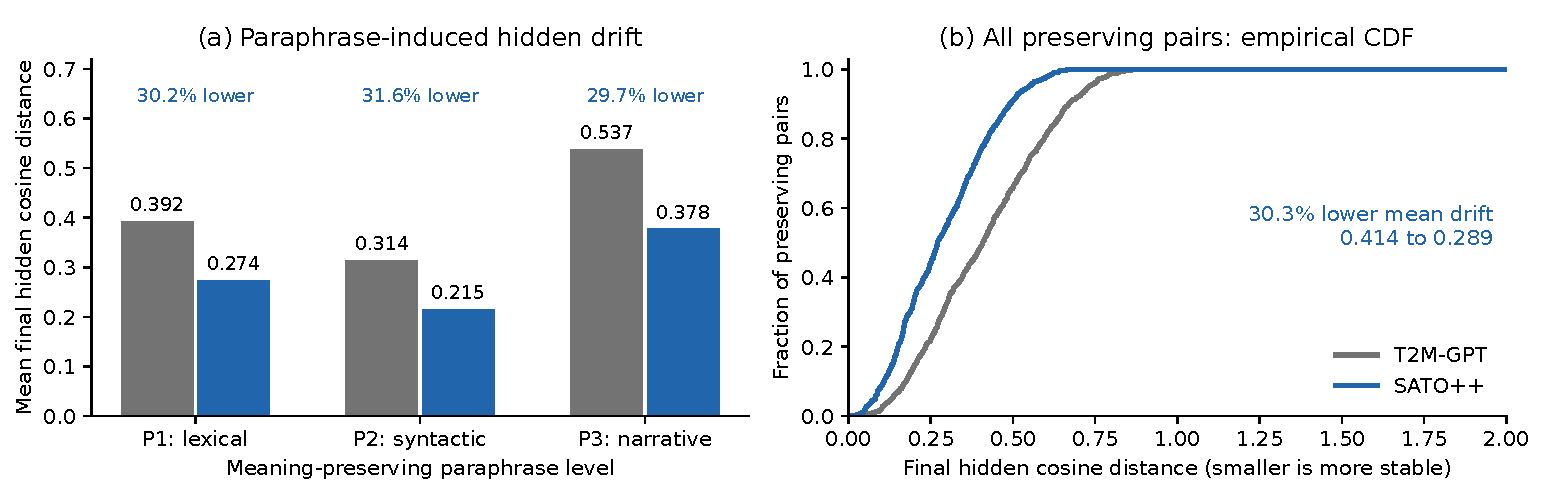
\includegraphics[width=\textwidth]{figures/paraphrase_latent_stability.pdf}
\caption{Lower hidden-state cosine displacement under preserving rewrites for the frozen-CLIP COMPASS checkpoint. The 900-pair diagnostic uses identical target prefixes and reports per-level means and the empirical cumulative distribution; it is separate from adapted-encoder generation evaluation.}
\label{fig:latent_stability}
\end{figure*}
\begin{figure*}[t]
\centering
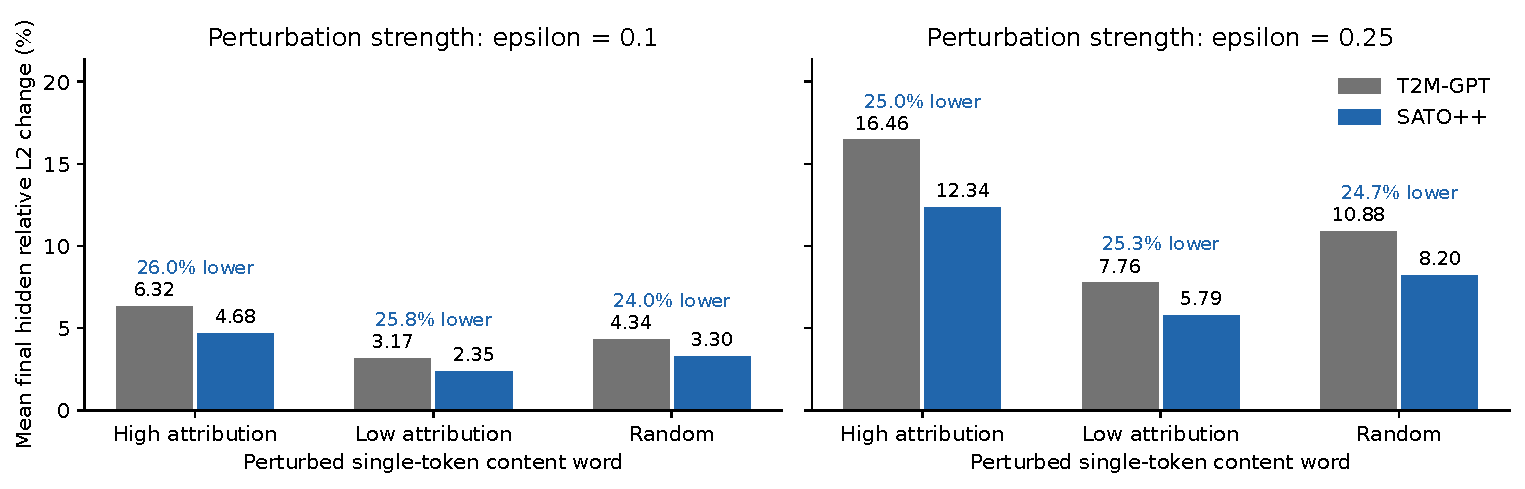
\includegraphics[width=\textwidth]{figures/attribution_guided_local_response.pdf}
\caption{Local input sensitivity on 100 shared groups. Interventions have norms 0.1 and 0.25 times the sentence-median content-word embedding norm. COMPASS has smaller mean relative responses in each condition. High/low ranks are model dependent; random-word identities and directions are shared.}
\label{fig:local_response}
\end{figure*}
The transfer test contains 364 P2 and 370 P3 pairs. HumanML3D-trained models
generate HumanML3D-format motion from KIT descriptions, using the frozen
HumanML3D evaluator throughout. With source encoders, COMPASS lowers FID$_D$
from 0.247 to 0.135 (Table~\ref{tab:human_to_kit}). With adapted encoders,
R@3$_P$ increases from 61.90\% to 70.31\% and paired embedding distance
decreases from 3.740 to 2.762, while first-token agreement decreases from
29.70\% to 24.66\%. Even within the adapted configuration, better embedding
alignment does not imply greater token agreement. Native FID/FID$_P$ are
omitted because no HumanML3D-format KIT real-motion reference is available.
This is text-domain transfer, rather than skeleton retargeting.

\subsection{Hidden-State Stability}
\label{sec:latent_diagnostics}
\begin{figure*}[t]
\centering
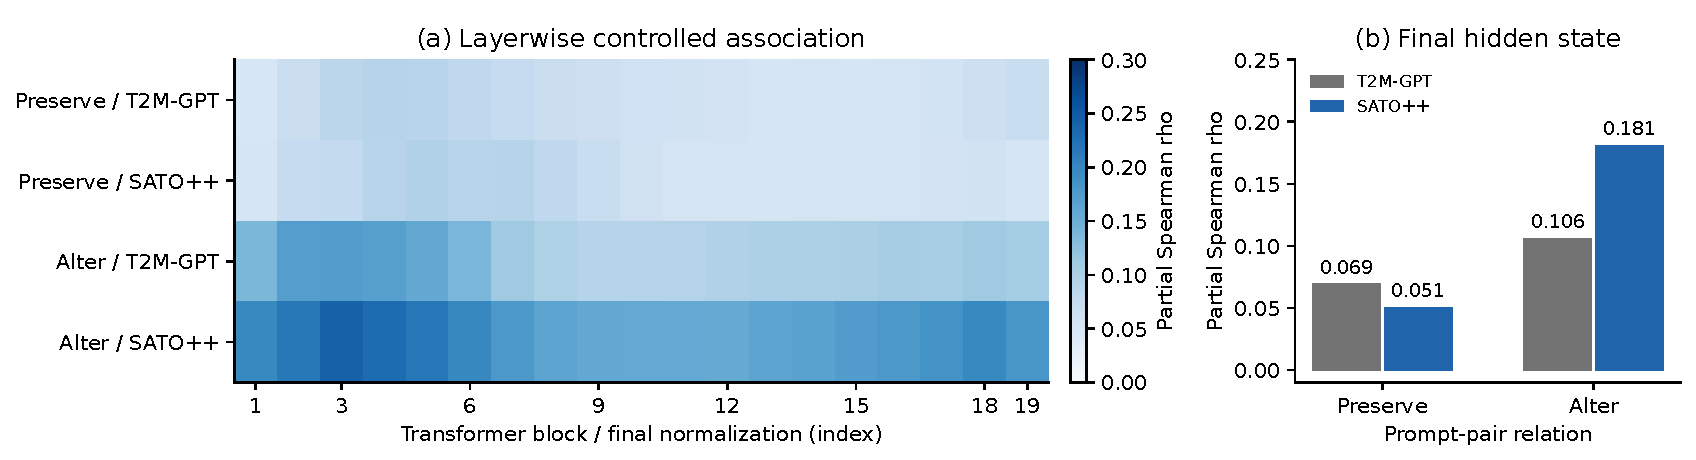
\includegraphics[width=\textwidth]{figures/relation_specific_association.pdf}
\caption{Association between attribution JSD and hidden-state cosine displacement for 900 preserving and 235 rule-edited pairs. (a) Partial rank correlations across 18 Transformer blocks and final normalization. (b) Final-state correlations. The between-model difference for altering pairs is uncertain; both panels use a common scale.}
\label{fig:attribution_association}
\end{figure*}
To examine internal sensitivity, we use the frozen-CLIP parent and a COMPASS
130k checkpoint before additional text adaptation. This mechanism analysis
retains the earlier training endpoint rather than the generation checkpoint
of Table~\ref{tab:humanml_methods}, so it characterizes the objective rather
than that specific row. The fixed HumanML3D subset
contains 300 held-out source-motion groups and 900 preserving pairs, one
P1/P2/P3 pair per group; original and mirrored motions share a group.
Both prompts receive the same teacher-forced target prefix. Mean final-state
cosine displacement over the first 16 valid positions decreases from 0.414
to 0.289 (30.3\%), with per-level reductions of 30.2\%, 31.6\%, and 29.7\%
(Figure~\ref{fig:latent_stability}).
On 100 shared groups, equal-norm interventions on high-attribution,
low-attribution, and random single-token words yield 24.0--26.0\% lower mean
relative hidden-state responses for COMPASS (Figure~\ref{fig:local_response}).
Both models remain more responsive to high- than low-attribution words.
Similar class-level reductions are compatible with shared local sensitivity
reduction in~\eqref{eq:theory_trace}, but do not prove the directional ordering
in~\eqref{eq:theory_contraction}: high/low positions are model dependent, and
continuous embedding interventions are not certified semantic-preserving edits.
The two experiments measure different quantities. Since
$1-\cos(a,b)=\|\bar a-\bar b\|_2^2/2$, a 30\% reduction in mean cosine
distance corresponds to approximately $1-\sqrt{0.70}=16.3\%$ reduction in
root-mean-square normalized chord length, not a 30\% reduction in mean
Euclidean distance. Section~\ref{sec:detail_attribution_details} examines
whether gradient connectivity and direct Jacobian estimates support a common
mechanism behind these observations.